\documentclass{fast_latex}

\usepackage[utf8]{inputenc}
\usepackage{lastpage}
\usepackage{setspace}
\usepackage{graphicx}
\usepackage[pdfborder={0 0 0}]{hyperref}		% turn on when latex is used (not miktec)
\usepackage{url} % LEO: urls \url{}
\usepackage{verbatim} % code and comment
\usepackage{longtable}
\usepackage{xspace}   % whitespace after a macro if no punctuation after the macro
\usepackage{multirow}
\usepackage{colortbl}
\usepackage{longtable}
\usepackage{array}
\usepackage{amssymb}
\usepackage{amsmath}

% This helps to get hyphenation in typewriter font (\texttt)
\usepackage[htt]{hyphenat}

\parindent0pt

\newcommand\deliverableNumber{D5.1.2}
\newcommand\deliverableTitle{User Manual of the FAST Catalogue}
\newcommand\deliverableTitleShort{Catalogue User Manual}
\newcommand\workpackageNumber{5}
\newcommand\workpackageTitle{Semantic catalogue of screen-flow resources and back-end Web Services}
\newcommand\authorOne{Ciprian Palaghita, Cyntelix}
\newcommand\authorTwo{Ismael Rivera, NUIG}
\newcommand\authorThree{Author 3}
\newcommand\authorFour{Author 4}
\newtheorem{example}{\emph{Example}}

\begin{document}
% explicit hyphenations
\hyphenation{RDF-Re-po-si-to-ry}
\hyphenation{name-space}

%\fontfamily{tahoma}\selectfont
\def\note#1{\marginpar{\footnotesize#1}} % use this to show the notes in the document
%\def\note#1{} % use this to hide the notes


\newenvironment{definition}{}{}

%%%%%%%%%%%%%%%%%%%%%%%%%%%%%%%%%%%%%%%%%%%%%%%%%%%%%%%%%%%%%%%%%%%%%%%%%%%%%%%%
% TITLE PAGES 
%%%%%%%%%%%%%%%%%%%%%%%%%%%%%%%%%%%%%%%%%%%%%%%%%%%%%%%%%%%%%%%%%%%%%%%%%%%%%%%%
\thispagestyle{empty}

% \pagenumbering{roman}

\begin{flushright}
	
\includegraphics[width=3cm]{images/FP7_logo}
\end{flushright}

\vspace{1cm}

%\begin{minipage}[p]{15cm}
	\begin{center}
		
\includegraphics{images/FAST_logo}\\
		\vspace{1cm}
		{\LARGE{\sffamily \emph{FAST AND ADVANCED STORYBOARD TOOLS}}}\\
		\vspace{0.5cm}
		{\LARGE \sffamily \emph{FP7-ICT-2007-1-216048}}\\
		\vspace{0.5cm}
		{\LARGE \sffamily \emph{http://fast.morfeo-project.eu}}\\
		\vspace{4cm}
		{\LARGE \sffamily \textbf{Deliverable \deliverableNumber}}\\
		\vspace{0.5cm}
		{\LARGE \sffamily \textbf{\deliverableTitle}}\\
		\vspace{2cm}
		{\large \sffamily \authorOne}\\
		\vspace{0.2cm}
		{\large \sffamily \authorTwo}\\
		\vspace{0.5cm}
		\vfill
		{\large \sffamily Date: 17/02/2011}\\
		\vspace{1cm}
		{\sffamily FAST is partially funded by the E.C. (grant code: FP7-ICT-2007-1-216048).}
		
	\end{center}
%\end{minipage}


\clearpage
%%%%%%%%%%%%%%
% NEXT PAGES %
%%%%%%%%%%%%%%
\pagestyle{scrheadings}

\lohead{
\includegraphics[width=4cm]{images/FAST_logo_transparent}}
%\cohead{\small\textcolor{fast@lightgrey}{\deliverableTitle}}
\rohead{\small{\today}}
%\lofoot{\small\textcolor{fast@lightgrey}{Task Force Ontologies}}
% \cofoot{\small{FAST 216048 --- \deliverableTitleShort}}
% \rofoot{\small{\thepage}}

\cofoot{\small{FAST $\bullet$ 216048 $\bullet$ \deliverableTitleShort{} $\bullet$ Page \thepage\ of \pageref{LastPage}}}


\newpage

\clearpage

\section*{Version History}

\begin{small}
\begin{tabular}{|l|l|l|p{6.6cm}|}
\hline
\rowcolor{fast@lightgrey}\textcolor{white}{\textbf{Rev. No.}} &
                         \textcolor{white}{\textbf{Date}} &
                         \textcolor{white}{\textbf{Author (Partner)}} &
                         \textcolor{white}{\textbf{Change description}}\\ \hline
1.0 & 19/02/2010 & Ciprian Palaghita (Cyntelix) & Release for M24 \\
 & & Ismael Rivera (NUIG) & \\ \hline
2.0 & 17/02/2011 & Ciprian Palaghita (Cyntelix) & Release for M36 \\
 & & Ismael Rivera (NUIG) & \\ \hline
\end{tabular}
\end{small}

\color{black}

\vfill
%{\bf Explanations of abbreviations on front page}\\
%\\
%%Nature \\
%R: Report \\
%P: Prototype \\
%R/P: Report and Prototype \\
%O: Other \\
% \\
%Dissemination level \\
%PU: Public \\
%PP: Restricted to other FP6 participants \\
%RE: Restricted to specified group \\
%CO: Confidential, only for NEPOMUK partners \\

\newpage

%%%%%%%%%%%%%%%%%%%%%
% Executive Summary %
%%%%%%%%%%%%%%%%%%%%%

\clearpage

\section*{Executive Summary}
\doublespacing

The present deliverable is intented to be the developer's manual of the prototype of the semantic catalogue. That said, whoever developing a component which will interact with the catalogue will find in this document a description of its architecture, the functionality provided together with the API (Application Programming Interface), data interchange formats, code errors and exceptions as well as several examples of usage.

\newpage

%%%%%%%%%%%%%%%%%%%%%
% Document Summary %
%%%%%%%%%%%%%%%%%%%%%

\clearpage

\section*{Document Summary}
% double spacing from here on:
\singlespacing

\begin{small}
\begin{tabular}
	%{| >{\columncolor{fast@lightgrey}}p{3.25cm}|p{6cm}|p{2cm}|p{2cm}|}
	{| >{\columncolor{fast@lightgrey}}p{3.25cm}|p{6cm}|p{2cm}|p{2cm}|}
	\hline
	\textcolor{white}{\textbf{Code}} & {FP7-ICT-2007-1-216048} & {\textbf{Acronym}} & {FAST}\\ \hline
	\textcolor{white}{\textbf{Full title}} & \multicolumn{3}{l|}{Fast and Advanced Storyboard Tools}\\ \hline
	\textcolor{white}{\textbf{URL}} & \multicolumn{3}{l|}{\url{http://fast.morfeo-project.eu}}\\ \hline
	\textcolor{white}{\textbf{Project officer}} & \multicolumn{3}{l|}{Annalisa Bogliolo}\\ \hline
\end{tabular}
\end{small}

\vspace{0.5cm}

\begin{small}
\begin{tabular}
	{| >{\columncolor{fast@lightgrey}}p{3.25cm}|p{1.25cm}|p{1cm}|p{1cm}|p{6.32cm}|}
	\hline
	\textcolor{white}{\textbf{Deliverable}} & {\textbf{Number}} & {\deliverableNumber} & {\textbf{Name}} & {\deliverableTitle}\\ \hline
	\textcolor{white}{\textbf{Work package}} & {\textbf{Number}} & {\workpackageNumber} & {\textbf{Name}} & {\workpackageTitle}\\ \hline
\end{tabular}
\end{small}

\vspace{0.5cm}

\begin{small}
\begin{tabular}
	{| >{\columncolor{fast@lightgrey}}p{3.25cm}|p{1.4cm}|p{3.2cm}|p{1.6cm}|p{3.37cm}|}
	\hline
	\textcolor{white}{\textbf{Delivery data}} & {\textbf{Due date}} & {28/02/2011} & {\textbf{Submitted}} & {25/02/2011}\\ \hline
	\textcolor{white}{\textbf{Status}} & \multicolumn{2}{l|}{} & \multicolumn{2}{l|}{final}\\ \hline
	\textcolor{white}{\textbf{Dissemination Level}} & \multicolumn{4}{l|}{Public $\boxtimes$ / Consortium $\square$}\\ \hline
	\textcolor{white}{\textbf{Short description of contents}} & \multicolumn{4}{p{10.85cm}|}{This deliverable is the technical documentation for the prototype developed as part of the WP5. It describes the catalogue's architecture, data interchange formats, APIs and examples of how to interact with it.}\\ \hline
	\textcolor{white}{\textbf{Authors}} & \multicolumn{4}{l|}{\authorOne}\\
	{} & \multicolumn{4}{l|}{\authorTwo}\\ 
%	{} & \multicolumn{4}{l|}{\authorOne}\\ 
%	{} & \multicolumn{4}{l|}{\authorOne}\\
  \hline
	\textcolor{white}{\textbf{Deliverable Owner}} & \multicolumn{2}{l|}{Cyntelix} & \textbf{email} & {cpalaghita@cyntelix.com} \\ \cline{4-5}
	\textcolor{white}{\textbf{(Partner)}} & \multicolumn{2}{l|}{} & \textbf{phone} & {+353 858494258} \\ \hline
	\textcolor{white}{\textbf{Keywords}} & \multicolumn{4}{p{10.85cm}|}{FAST, semantic catalogue, gadget catalogue, RDF store}\\ \hline
\end{tabular}
\end{small}

\newpage

%%%%%%%%%%%%%%%%%%%%%
% TABLE OF CONTENTS %
%%%%%%%%%%%%%%%%%%%%%
\doublespacing
\setcounter{tocdepth}{2}
\tableofcontents
\cleardoublepage
% \pagenumbering{arabic}

\clearpage
\listoftables

\clearpage
\listoffigures

%%%%%%%%%%%%%%%%%%%%%%%%%
% BEGINNING OF SECTIONS %
%%%%%%%%%%%%%%%%%%%%%%%%%
% \rofoot{\small{Page \thepage\ of \pageref{LastPage}}} 

\clearpage
\section{Introduction} % (fold)
\label{sec:introduction}
This section starts establishing the goal and scope of the present document, shows how it is structured and details the relation to others documents and work packages.

\subsection{Goal and Scope} % (fold)
\label{sub:goal_and_scope}

This is an introductory manual for developers who want to adopt and use the FAST semantic catalogue. It explains the main functionalities implemented so far, an overview of its architecture and a detailed \emph{Application Programming Interface} or API of the complete set of the operations offered through a REST service.

% subsection goal_and_scope (end)

\subsection{Structure of the document} % (fold)
\label{sub:structure_of_the_document}

The deliverable presents both the external and internal architecture in Section~\ref{sec:architecture_overview}, then in Section~\ref{sec:catalogue_api} it is detailed the Catalogue API, query formats, interchange formats, error codes and so on.

% subsection goal_and_scope (end)

\subsection{Changes from previous version} % (fold)
\label{sub:changes_from_previous_version}

This sections enumerates and gives a brief overview of the changes made in the deliverable with regards to the version 1.0 released for the milestone M24.

\begin{itemize}
 \item The installation guide has been modified to include some minor changes in the configuration, and a better example for the ``Hello World!''.
 \item Two operations have been removed: 'Find' and 'Check' for screens, used at screen-flow design, since the same functionaly was offered by the operation Find\&Check, so no functionality is duplicated or overlapped. However, using this unique operation does not mean that every request does a \emph{find} and a \emph{check}, these actions are optional and can be specified in the request.
 \item There have been some substantial changes in the API methods Find\&Check and Planner and Metadata reflect the changes made in the Catalogue prototype.
 \item There have been created new operations in the API to support the prototype-based semantics for RDF as defined in D2.2.3~\cite{moeller2011fast_ontology}.
 \item The Catalogue Architecture has been updated to reflect the new functionality and other changes.
 \item There have been implemented new mechanisms for managing and importing ontologies. These mechanism are explained in~\ref{ssec:logic_tier}.
 \item A new appendix has been added in order to explain the decisions and logic behind the main methods of the API, how the building block recommendation works, algorithm supporting the building block planning, matching and inferencing in pre-/post-conditions, and the integration with iServe\footnote{http://iserve.kmi.open.ac.uk/}, enhancing the web service discovery.
 \item There are two new resources, and its CRUD operations: concepts (classes) and samples (instances).
\end{itemize}

% subsection changes_from_previous_version (end)

% section introduction (end)

\clearpage
\section{Installation Guide} % (fold)
\label{sec:installation_guide}

This section provides instructions on how to manually install and configure the FAST Catalogue. The first part of this guide presents some requirements to be considered before the installation, then it gives broad general instructions, and the last part contains a more detailed installation notes for specific configurations.

\subsection{System Requirements} % (fold)
\label{sub:system_requirements}

In addition to the software itself, a standard FAST Catalogue installation has the following requirements:
\begin{itemize}
  \item Java\footnote{http://java.sun.com/} (version 6 or later) is required to run the software.
  \item A Java Servlet Container that supports Java Servlet API 2.4 and Java Server Pages (JSP) 2.0, or newer. We recommend using a recent, stable version of Apache Tomcat\footnote{http://tomcat.apache.org/}. At the time of writing, this is either version 5.5.x or 6.x.
\end{itemize}

In addition, there are various optional dependencies which are required if you want to use certain advanced features (see Section~\ref{sub:installation_instructions}).

% subsection system_requirements (end)

\subsection{Obtaining the FAST catalogue} % (fold)
\label{sub:obtaining_the_fast_catalogue}

It is recommended to have a Subversion client installed before you download the code (although you can theoretically download files without Subversion, this would mean tediously downloading each individual file manually). The recommended software is the official Subversion client, available from the Subversion project page\footnote{http://subversion.tigris.org/}. Note that this client uses a command-line interface, which the instructions below use. Alternatively, you can get subversioning software with a graphical user interface such as TortoiseSVN.

To download from the latest release (recommended), enter the following command from the command-line in the directory you wish to download to:
\begin{verbatim}
svn checkout https://svn.forge.morfeo-project.org/fast-fp7project/trunk/catalogue_service
\end{verbatim}

% subsection obtaining_the_fast_catalogue (end)

\subsection{Installation Instructions} % (fold)
\label{sub:installation_instructions}

Once you have got the source code, first step should be addressed is its compilation. You may manually compile the source yourself, however the FAST Catalogue comes along with a script to facilitate this task. This script has been made using a Java build tool called Ant \footnote{http://ant.apache.org/}. Hence, we recommended to get and install such a tool in order to follow the instructions below.

Now you can compile, package and run the application via:
\begin{verbatim}
ant clean
ant prepare
ant compile
\end{verbatim}

Or using a task which gather the previous three tasks and creates WAR file ready to distribute or deploy:
\begin{verbatim}
ant dist
\end{verbatim}

After executing with no errors this task, a WAR file should have been created in the /dist directory. A WAR file, which stands for  Web Application Archive, is just a JAR file used to distribute a collection of JavaServer Pages, servlets, Java classes, XML files, tag libraries and static Web pages (HTML and related files) that together constitute a Web application, in this case, the FAST Catalogue.

Note that it is also possible to get the compiled WAR file directly from the SVN server. This file can be located at \url{https://svn.forge.morfeo-project.org/fast-fp7project/distribution/catalogue}.

Then, last step is to deply the WAR file into the servlet container. If the server chosen was Apache Tomcat, the procedure for deploying a Web application is:
\begin{enumerate}
	\item Stop Tomcat.
	\item Delete existing deployment. If you have previously deployed "foo.war" in TOMCAT\_HOME/webapps, then it has been unpacked into webapps/foo/... You must delete this directory and all its contents. On Unix, this can be done with
rm -r \$TOMCAT\_HOME/webapps/foo
	\item Copy WAR file to TOMCAT\_HOME/webapps/.
	\item Start Tomcat.
\end{enumerate}

Now you have successfully built the FAST catalogue, however we highly recommend you to read Section~\ref{sub:configuration} and tune your FAST Catalogue instance.

% subsection installation_instructions (end)

\subsection{Configuration} % (fold)
\label{sub:configuration}

The following section covers the configuration options you may have to set up before start using the Catalogue. The configuration is done in the file \emph{repository.properties} in the root directory where the Catalogue has been deployed.

The resources (building blocks) created in the Catalogue have an unique identifier or URI. This URI is constructed relatively to the Catalogue URL which is configured by the parameter \emph{serverURL}. If you are testing the application in your machine, it may look like \verb|http://localhost:8080/FASTCatalogue|.

The FAST Catalogue relies on a Sesame repository for the persistent storage. Sesame repositories can be \emph{local} or \emph{remote}. Local repositories just need the parameter \emph{storageDir} pointing at a local directory, with write permission in order to allow Sesame to create and delete the necessary binary files to store and retrieve the data.

\begin{verbatim}
storageDir=/opt/fast-catalogue/repository
\end{verbatim}

Setting up a remote repository requires a few more steps. \emph{Remote} means the repository is installed in a web server and accessed via HTTP, independently if it is in the same machine or in a different dedicated machine. First the OpenRDF Sesame Server needs to be installed. The installation guide of this server is detailed in the Chapter 5 and 6 of the User Guide for Sesame 2.2 \cite{sesame2.2}. Once the Sesame server is deployed, and a repository has been created, the parameters sesameServer and repositoryID will take the values of the Sesame server URL and the repository identifier.

\begin{verbatim}
sesameServer=http://sesameServerURL/openrdf-sesame
repositoryID=repository-id
\end{verbatim}

Note: If you want to provide the data of in the repository via a SPARQL endpoint, the easiest way it is to configure the Catalogue using a remote repository, as in this case Sesame provides an HTTP accessible SPARQL endpoint by default.


% subsection installation_instructions (end)

\subsection{Hello World!} % (fold)
\label{sub:hello_world}

It is recommended to check if the FAST Catalogue has been successfully installed. The simpliest manner is to send a HTTP GET request to retrieve concepts (classes) and attributes (properties) of the predefined ontologies to \verb|http://catalogueURL/FASTCatalogue/concepts| (e.g. typing the address in a Web browser). The response is a list of all the concepts and their associated metadata, as in the following example:

\singlespacing
\begin{verbatim}
[
  {
    "attributes": [],
    "label": {"en": "A request to search for an item"},
    "tags": [{
      "label": {"en": "amazon"},
      "means": "http://www.amazon.com"
    }],
    "uri": "http://fast.morfeo-project.org/ontologies/amazon#SearchRequest"
  },
  {
    "attributes": [
      {
        "type": "http://xmlns.com/foaf/0.1/Document",
        "uri": "http://fast.morfeo-project.org/ontologies/amazon#smallImage"
      },
      {
        "type": "http://www.w3.org/2001/XMLSchema#double",
        "uri": "http://fast.morfeo-project.org/ontologies/amazon#price"
      }
    ],
    "label": {"en": "An item handled by the Amazon Service"},
    "tags": [{
      "label": {"en": "amazon"},
      "means": "http://www.amazon.com"
    }],
    "uri": "http://fast.morfeo-project.org/ontologies/amazon#Item"
  },
  ...
]
\end{verbatim}
\doublespacing

By default, the Catalogue does not include any building block, therefore any GET request for any type of building block, as for instance to \verb|http://catalogueURL/FASTCatalogue/screens| should return an empty list \verb|[]| (if JSON requested) or \verb|No screens found| (if HTML requested).

% subsection hello_world (end)

% section installation_guide (end)


\clearpage
\section{Architecture Overview} % (fold)
\label{sec:architecture_overview}

This sections presents a technical overview of the Catalogue's architecture (see Figure~\ref{fig:catalogue_architecture}), and how the interaction with external applications or APIs is done. The Catalogue platform has a modular design, which are spread in basically three layers, depending on the nature of each component:
\begin{itemize}
 \item \emph{Presentation tier} is the top layer which represents the public API for the Catalogue. It brings together all the relaying functionality in a simple but flexible manner to be used by other IDEs or applications. In FAST, this is the unifying interface with other components such as the Gadget Visual Storyboard or the Service Wrapper.
 \item \emph{Logic tier} is the core layer which implements the business logic for the different processes involved in the Catalogue, and communicates with third party libraries or APIs.
 \item \emph{Data tier} is the bottom layer. It offers storage capabilities in triple stores, relational databases and binary files, and acts as an abstraction to RDF model logic.
\end{itemize}

\begin{figure}[htb]
\label{fig:catalogue_architecture}
\begin{center}
	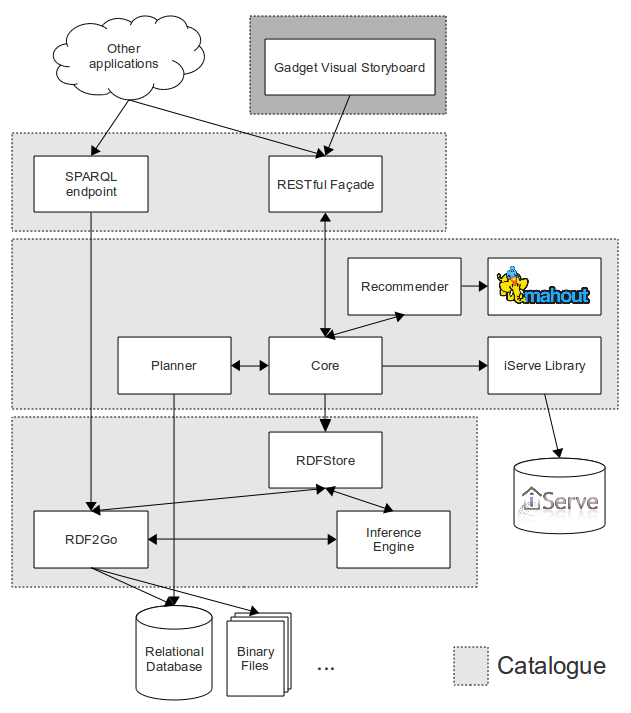
\includegraphics[width=13cm]{images/catalogue_architecture}
	\caption{Catalogue's Architecture}
\end{center}
\end{figure}

\subsection{Presentation tier / Public API}

The Presentation tier is the public interface or API of the Catalogue. The main purpose of this layer is to provide its functionality to the Gadget Visual Storyboard, or any other third party IDE or application. The API is offered in a REST (REpresentational State Transfer) style, making it easy to consume than other complex APIs. REST is an architectural style, not a toolkit or a standard , even though, it makes use of standards like HTTP, URI, Resource Representations or MIME types. Another characteristic of the REST style is its stateless assumption. The Catalogue adopts this strategy; therefore every request needs a complete set of information in order to prepare the response. The API provided is explained in detail in Section~\ref{sec:catalogue_api}.

As part of the Presentation tier, a SPARQL endpoint has been implemented using the SPARQL protocol service as defined in the SPROT \cite{sprot} specification. The SPARQL endpoint is mostly offered to enable other developers to query directly the Catalogue knowledge base using SPARQL queries. This feature is supported by the Sesame RESTful HTTP interface for SPARQL Protocol for RDF.

\subsection{Logic tier}
\label{ssec:logic_tier}

The Logic tier or business logic layer contains all the FAST domain-specific processing. The resources and relations between each other, which define the domain model, are extracted from the FAST ontology~\cite{moeller2011fast_ontology}. This layer provides support to the functions defined in the API, and interact with the data tier to retrieve and store any information of the data model.

This layer provides several mechanisms to search and browse these different resources. To know more about these capabilities, please read Sections~\ref{ssub:screen_findcheck},~\ref{ssub:screen_component_findcheck} and~\ref{sub:planning} where the API calls are defined, and Appendix F for more details about the implementation.

At the bottom level of the Gadget Architecture~\cite{reyes2011gadget_architecture} are the back-end services. These are RESTful services, SOAP-based web services, or similar. In FAST, these web services are wrapped, extracting their definition and encapsulating their behaviour. The creation of these service wrappers is on demand, and the input for this process is a particular definition of a web service. However, the Catalogue does not crawl the Web looking for Web services. Instead, and to enrich the collection of available web services, the Catalogue integrates and queries iServe, a platform for publishing Semantic Web Services as linked data, no matter their original format. Therefore, thousands of web services defined or annotated in a semantic way, are also served from the Catalogue, in a uniform manner.

The Catalogue is a semantic application. As a consequence, it must handle and work with ontologies and vocabularies. The business model itself is described by in the FAST ontology, and the Catalogue goes along with a few established ontologies integrated in its core (see~\cite{moeller2011fast_ontology}). However, the definition of the pre-/post-conditions of the building blocks are open to any ontology or vocabulary, and they may reference classes and properties from any of them. To have a better understanding of these classes, properties, and so on, the Catalogue needs to import into its own knowledge base the ontology in which they are described along with the relations with other classes and properties. In order to adquire these vocabularies, it follows the basic recipe dictated in~\cite{berrueta2008} which says that deferencing a vocabulary URI should provide a machine-processable (RDF) content back. Nonetheless, this is just a good practice and not every ontology published on the Internet follows it. Hence, going a step further, whenever an ontology cannot be retrieved by deferencing its URI, the Catalogue queries Sindice\footnote{http://www.sindice.com/}, a semantic search engine, which crawls and contains thousands of vocabularies and metadata as their provenance, which the Catalogue can take advantage of.


\subsection{Data tier}

The Data tier abstracts the interaction with triple stores, RDF models and physical persistence to disk, database, etc. It provides different mechanisms to allow the Catalogue the storage of domain objects into a triple store in its underlying representation of RDF.

There are many triple stores solutions, all of them with their own advantages and disadvantages. To make the Catalogue independent of the solution adopted, it makes uses of RDF2Go, an abstraction over triple (and quad) stores. The RDF2Go API allows interacting with the semantic representation of the model (triples) in a generic manner, and also brings the flexibility of choosing different triple stores to persist them.

The current implementation of the Catalogue prototype at M36 uses Sesame 2 as triple store. This solution has a wide community behind, and it has attractive advantages such as being completely extensible and configurable regarding to storage mechanisms, inferencers, RDF file formats, query result formats and query languages.


% section architecture_overview (end)


\clearpage
\section{Catalogue API} % (fold)
\label{sec:catalogue_api}

This section provides a high-level overview of the Catalogue API. It describes the calls or operations supported, specific parameters and responses for each operation, supported interchange formats and some examples to facilitate the understanding of the API.


\subsection{JSON Interchange Format} % (fold)
\label{sec:json_interchange_format}

The body of the requests to the API must be in JSON\footnote{http://www.json.org/}. JSON is a lightweight data interchange format which simplicity has resulted in widespread use among web developers, easy to read and write and able to process and parse using any programming language because its structures map directly to data structures used in most programming languages.

Every HTTP request should be encoded using the MIME type \texttt{application/json} and the charset \texttt{UTF-8}.

The following is an example of a Find \& Check request:

\singlespacing
\begin{verbatim}
{
  "canvas": [
    { "uri": "http://catalogueURL/screens/clones/2338" },
    { "uri": "http://catalogueURL/screens/clones/1323" }
  ],
  "palette": [
    { "uri": "http://catalogueURL/screens/636" }
  ],
  "domainContext": {
    "tags": [
      {
        "label": { "en-GB": "Amazon" },
        "means": "http://dbpedia.org/page/Amazon.com"
      }
    ],
    "user": "http://ismaelrivera.es/#me",
  },
  "criterion": "reachability"
}
\end{verbatim}
\doublespacing

\subsubsection{Internationalisation I18n} % (fold)

In order to offers an adaptable solution to various languages and regions without major engineering changes, internationalisation is considered from an early stage in the catalogue development. Underlying representation technologies used to develop the catalogue (RDF/XML and JSON) allow to implement this feature. This feature is implemented by the addition of a language tag to every 'string' desired. The specification of this language tag is composed by the language code and the country code, following the ISO 639\footnote{http://ftp.ics.uci.edu/pub/ietf/http/related/iso639.txt} for languages and the ISO 3166\footnote{http://userpage.chemie.fu-berlin.de/diverse/doc/ISO\_3166.html} for countries. The following example illustrates how to use it properly in both formats.

\singlespacing
\begin{verbatim}
{
  "label": {
    "en-GB": "Product Search",
    "es-ES": "Búsqueda de productos",
    "de-DE": "Produktsuche"
  },
  "description": {
    "en-GB": "On this screen, the user can enter a search term.",
    "es-ES": "En esta ventana, el usuario puede introducir el criterio de búsqueda",
    "de-DE": "Auf diesem Screen kann der Benutzer einen Suchbegriff eingeben."
  }
}
\end{verbatim}
\doublespacing

\singlespacing
\begin{verbatim}
<rdf:RDF
    xmlns:rdf="http://www.w3.org/1999/02/22-rdf-syntax-ns#"
    xmlns:foaf="http://xmlns.com/foaf/0.1/"
    xmlns:dc="http://purl.org/dc/terms/"
    xmlns:fgo="http://purl.oclc.org/fast/ontology/gadget#"
    xmlns:xsd="http://www.w3.org/2001/XMLSchema#"
    xmlns:rdfs="http://www.w3.org/2000/01/rdf-schema#"
    xmlns:ctag="http://commontag.org/ns#">
  <rdf:Description rdf:about="http://catalogueURL/screens/1">
    <rdf:type rdf:resource="http://purl.oclc.org/fast/ontology/gadget#Screen"/>
    <rdfs:label xml:lang="en-gb">Product Search</rdfs:label>
    <rdfs:label xml:lang="en-es">Búsqueda de productos</rdfs:label>
    <rdfs:label xml:lang="en-de">Produktsuche</rdfs:label>
    <dc:description xml:lang="en-gb">On this screen, the user can enter a search
    term.</dc:description>
    <dc:description xml:lang="en-gb">En esta ventana, el usuario puede introducir
    el criterio de búsqueda.</dc:description>
    <dc:description xml:lang="en-gb">Auf diesem Screen kann der Benutzer einen
    Suchbegriff eingeben.</dc:description>
  </rdf:Description>
</rdf:RDF>
\end{verbatim}
\doublespacing

Internationalisation is being used by the attributes \emph{label} and \emph{description} of any building block, \emph{label} of the pre-/post-conditions and \emph{label} of the tags.

% subsection json_interchange_format (end)

\subsection{Linked Data} % (fold)
\label{sub:linked_data}

Apart from serving as the back-end system for the Gadget Visual Storyboard (GVS), the catalogue publishes all FAST building blocks as linked data, following the principles as originally defined in \cite{bernersLee2006linkedData}, in order to make them available to arbitrary third party applications. Each building block is identified by an HTTP URI and hosted through the catalogue so that it can be dereferenced through the same URI. For each building block, data is available in representations in different standard formats such as JSON (for communication with the GVS), RDF/XML, Turtle, or even HTML+RDFa as a human-readable version. 
Following the principles and best practices proposed in \cite{berrueta2008} and \cite{sauermann2008cool_uris}, these representations are served based on the request issued by the requesting agent, using a technique called \emph{content negotiation}.
As required by the forth rule of linked data, individual building blocks link to other data on the Web, thereby preventing so-called isolated ``data islands''.

In order to understand how content negotiation is implemented in the catalogue, a few concepts need to be understood. The URI of a particular building block must be understood as the identifier of the building block such, as opposed to a particular representation (JSON, HTML, etc.) of it. In fact, each such representation has its own URI, under which it can be retrieved. Using the terminology established in \cite{w3c2004webArchitecture}, the building block is a \emph{non-information resource}, whereas each representation is an \emph{information resource}. In the process of content negotiation, the requesting agent will first request the URI of the building block as such (e.g., \verb|http://catalogueURL/screens/235|), as well as the required representation format (e.g., JSON). The catalogue will then inspect the request and redirect the requester to the appropriate representation (e.g., \verb|http://catalogueURL/screens/235.json|), as illustrated in Fig.~\ref{fig:content_negotiation}.
On the Web, different representations for the same resource are called \emph{variants}, and content negotiation is the mechanism used to determine which of the representations is most appropriate for a given request.

\begin{figure}[htb]
\label{fig:content_negotiation}
\begin{center}
	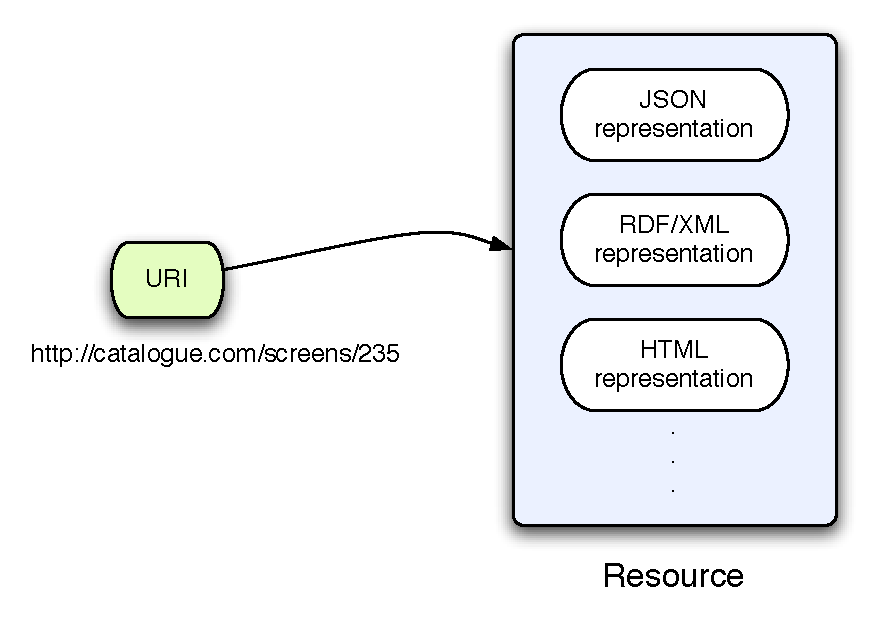
\includegraphics[width=12cm]{images/content_negotiation}
	\caption{Content Negotiation}
\end{center}
\end{figure}

In summary, the basic idea of content negotiation, as stated in the \cite{http1.1}, is to serve the best variant for a resource, taking into account what variants are available, what variants the server may prefer to serve, what the client can accept, and with which preferences. In HTTP, this is done by the client which may send, in its request, accept headers (\texttt{Accept}, \texttt{Accept-Language} and \texttt{Accept-Encoding}), to communicate its capabilities and preferences in format, language and encoding, respectively.

In fact, what the catalogue really does is ``format negotiation'' since the alternate representations are just based on the selection of the media type, through the accept header, but does not consider different languages or encoding types. The formats supported are JSON, RDF/XML, Turtle and HTML+RDFa. Even though the accept header is desired, the different representations can also be retrieved directly by dereferencing their own URI. The convention used in the catalogue for deriving a representation URI from a building block URI is to simply attach a matching suffix, such as \texttt{.rdf}, \texttt{.ttl}, \texttt{.json} or \texttt{.html} for RDF/XML, Turle, JSON or HTML respectively.

Lastly, content negotiation needs to identify which player is going to take the lead on it. There are two kinds of content negotiation which are possible in HTTP: server-driven and agent-driven negotiation. The approach followed by the catalogue is agent-driven negotiation, hence selecting a specific representation for a resource is responsibility of the user agent. If none is specified, by default, the server will choose the JSON representation.

% subsection content_negotiation (end)

\subsection{API calls} % (fold)
\label{sub:api_calls}

The Catalogue API is a programmatic interface into many of the Catalogue's features. It includes not only control over creation, modification and deletion of building blocks, but it has been extended to support advanced search and recommendation capabilities.

This section contains detailed descriptions of the operations permitted by the API, detailing request parameters, response elements, any special errors and examples of requests and responses. The URL format is also specified for each operation, where \emph{catalogueURL} has to be replaced for the real URL the service is installed (e.g. http://demo.fast.morfeo-project.org/catalogue).

\subsection{Managing building blocks} % (fold)
\label{sub:managing_building_blocks}

Any building block within the Catalogue is a resource in terms of REST philosophy, therefore it can be created, retrieved, modified or deleted, using a certaing URL and a specific HTTP method for every operation. Two concepts should be clarified: \emph{collection}, as a set of resources are accessed at the URL \verb|http://catalogueURL/[type]| where \emph{catalogueURL} is  where the Catalogue server is installed and \verb|[type]| is the plural of the name of the building block (e.g. screens, operators), and \emph{member} of the collection, in other words, the building block itself, being accessed at the URL \verb|http://catalogueURL/[type]/[id]| where \verb|[id]| has to be replaced by the identifier of a specific building block. The details of the operations and which HTTP verb has to be used can be found in the Table~\ref{tab:crud_operations}.

\begin{table}[htb!]
\caption{CRUD operations}
\label{tab:crud_operations}
\begin{center}
\begin{tabular}{|p{2.5cm}|p{2.5cm}|p{3.5cm}|p{5cm}|}
\hline
\rowcolor{fast@lightgrey}\textcolor{white}{Resource} &
                         \textcolor{white}{HTTP method} &
                         \textcolor{white}{HTTP body} &
                         \textcolor{white}{Description}\\ \hline
Collection URI & GET & N/A & \textbf{List} the members of the collection.\\ \hline
Collection URI & PUT & N/A & Not used.\\ \hline
Collection URI & POST & JSON representation of the building block & \textbf{Create} a new entry in the collection where the URI is assigned automatically by the collection. The URI created is returned by this operation.\\ \hline
Collection URI & DELETE & N/A & Not used.\\ \hline
Member URI & GET & N/A & \textbf{Retrieve} the addressed member of the collection.\\ \hline
Member URI & PUT & JSON representation of the building block & \textbf{Update} the addressed member of the collection or create it with a defined URI.\\ \hline
Member URI & POST & N/A & Not used. \\ \hline
Member URI & DELETE & N/A & \textbf{Delete} the addressed member of the collection.\\ \hline
\end{tabular}
\end{center}
\end{table}

The JSON structure for creating any building block can be found in the appendixes. All of them are composed of a common structure which can be found in Section Appendix B, and some specific information depending on the type. Screen-flows are defined in Appendix C, screens in Appendix D and forms, operators and back-end services share the same structure detailed in Appendix E. However, a few examples of request and responses are shown in order to clarify how the requests are constructed and sent, and how the responses look like.

To create a new screen, a POST request is sent to the catalogue server, concretely to \texttt{http://cata\-logueURL/screens}, including the JSON representation of the screen in the body of the request:

\singlespacing
\begin{verbatim}
{
  "code": "http://demo.fast.morfeo-project.org/code/amazonList.js",
  "creationDate": "2010-01-26T17:01:13+0000",
  "creator": "http://ismaelrivera.es/#me",
  "description": {"en-gb": "Please fill the description..."},
  "homepage": "http://fast.morfeo-project.eu/",
  "icon": "http://demo.fast.morfeo-project.org/images/amazonList.png",
  "id": "28",
  "label": {"en-gb": "Amazon Product List"},
  "postconditions": [
    {
      "id": "item",
      "label": { "en-gb": "An item" },
      "pattern": "?item 
                  http://www.w3.org/1999/02/22-rdf-syntax-ns#type
                  http://fast.morfeo-project.org/ontologies/amazon#Item",
      "positive": "true"
    }
  ],
  "preconditions": [
    {
      "id": "filter",
      "label": { "en-gb": "A search request" },
      "pattern": "?search
                  http://www.w3.org/1999/02/22-rdf-syntax-ns#type
                  http://fast.morfeo-project.org/ontologies/amazon#SearchRequest",
      "positive": "true"
    }
  ],
  "rights": "http://creativecommons.org/",
  "screenshot": "http://demo.fast.morfeo-project.org/images/amazonProductList.png",
  "tags": [{"label": {"en-gb": "amazon"}}],
  "version": "1.0"
}
\end{verbatim}
\doublespacing

The URI of the screen is created using the id specified in the JSON request. So, the response for this operation is:

\singlespacing
\begin{verbatim}
{
  "code": "http://demo.fast.morfeo-project.org/code/amazonList.js",
  "creationDate": "2010-01-26T17:01:13+0000",
  "creator": "http://ismaelrivera.es/#me",
  "description": {"en-gb": "Please fill the description..."},
  "homepage": "http://fast.morfeo-project.eu/",
  "icon": "http://demo.fast.morfeo-project.org/images/amazonList.png",
  "id": "28",
  "label": {"en-gb": "Prueba1"},
  "postconditions": [
      {
        "id": "item",
        "label": { "en-gb": "An item" },
        "pattern": "?item
                    http://www.w3.org/1999/02/22-rdf-syntax-ns#type
                    http://fast.morfeo-project.org/ontologies/amazon#Item",
        "positive": "true"
      }
    ]
  ],
  "preconditions": [
    [
      {
        "id": "filter",
        "label": { "en-gb": "A search request" },
        "pattern": "?search
                    http://www.w3.org/1999/02/22-rdf-syntax-ns#type
                    http://fast.morfeo-project.org/ontologies/amazon#SearchRequest",
        "positive": "true"
      }
    ]
  ],
  "rights": "http://creativecommons.org/",
  "screenshot": "http://demo.fast.morfeo-project.org/images/amazonProductList.png",
  "tags": [{"label": {"en-gb": "amazon"}}],
  "uri": "http://catalogueURL/screens/28",
  "version": "0.1"
}
\end{verbatim}
\doublespacing

To obtain all the screens stored in the catalogue a HTTP GET request is sent to the Collection URI and the response may be something like this:

\singlespacing
\begin{verbatim}
[
  {
    "code": "http://demo.fast.morfeo-project.org/code/amazonList.js",
    "creationDate": "2010-01-26T17:01:13+0000",
    "creator": "http://ismaelrivera.es/#me",
    "description": {"en-gb": "Please fill the description..."},
    "homepage": "http://fast.morfeo-project.eu/",
    "icon": "http://demo.fast.morfeo-project.org/images/amazonList.png",
    "id": "28",
    "label": {"en-gb": "Prueba1"},
    "postconditions": [
      [
        {
          "id": "item",
          "label": { "en-gb": "An item" },
          "pattern": "?item
                      http://www.w3.org/1999/02/22-rdf-syntax-ns#type
                      http://fast.morfeo-project.org/ontologies/amazon#Item",
          "positive": "true"
        }
      ]
    ],
    "preconditions": [
      [
        {
          "id": "filter",
          "label": { "en-gb": "A search request" },
          "pattern": "?search
                      http://www.w3.org/1999/02/22-rdf-syntax-ns#type
                      http://fast.morfeo-project.org/ontologies/amazon#SearchRequest",
          "positive": "true"
        }
      ]
    ],
    "rights": "http://creativecommons.org/",
    "screenshot": "http://demo.fast.morfeo-project.org/images/amazonProductList.png",
    "tags": [{"label": {"en-gb": "amazon"}}],
    "uri": "http://catalogueURL/screens/28",
    "version": "0.1"
  },
  {
    "creationDate": "2011-02-07T09:59:52+0000",
    "creator": "fabio",
    ...,
    "uri": "http://catalogueURL/screens/14",
    "version": "1.0"
  },
  {
    "creationDate": "2011-02-07T09:59:52+0000",
    "creator": "javier",
    ...,
    "uri": "http://catalogueURL/screens/564",
    "version": "1.0"
  }
]
\end{verbatim}
\doublespacing


\subsection{Managing concepts (classes) and attributes (properties)} % (fold)
\label{sub:managing_concepts_attributes}

This method allows the creation of new classes and properties which do not belong to any existing ontology or vocabulary. The URI of this new class has the Catalogue URL as prefix, in order to be dereferenceable, followed by a domain, which groups these classes, and a name (http://catalogueURL/concepts/[domain]/[name]).

The URL for this operation is \verb|http://catalogueURL/concepts|.

The concepts are another type of resource, hence the common CRUD operations (GET to retrieve, POST to create, PUT to update and DELETE to remove) are supported for them.

Example of concept:

\singlespacing
\begin{verbatim}
{          
  "description": {"en-gb": "Represents a school with its coordinates."}, 
  "label": {"en-gb": "School"},
  "tags":[{
    "label": {"en-gb": "school"}
   }],
  "subclassOf": "http://www.w3.org/2003/01/geo/wgs84_pos#SpatialThing",
  "attributes": [
    {
      "uri": "http://www.w3.org/2003/01/geo/wgs84_pos#lat",
      "type": "http://www.w3.org/2001/XMLSchema#double"
    },
    {
      "uri": "http://www.w3.org/2003/01/geo/wgs84_pos#long",
      "type": "http://www.w3.org/2001/XMLSchema#double"
    }
  "name": "school",
  "domain": "institutions"
}
\end{verbatim}
\doublespacing


\subsection{Managing samples/instances of concepts} % (fold)
\label{sub:managing_samples}

It is allowed to create instances of classes, or so-called samples of concepts. The samples are another type of resource, hence the common CRUD operations (GET to retrieve, POST to create, PUT to update and DELETE to remove) are supported for them.

Example of sample:

\singlespacing
\begin{verbatim}
{
  "concept": "http://catalogueURL/concepts/institutions/school",
  "attributes": [
    {
      "uri": "http://www.w3.org/2003/01/geo/wgs84_pos#lat",
      "value": "60.025"
    },
    {
      "uri": "http://www.w3.org/2003/01/geo/wgs84_pos#long",
      "value": "34.224"
    }
}
\end{verbatim}
\doublespacing


\subsubsection{Prototype cloning} % (fold)
\label{ssub:prototype_cloning}

The resources created by the requests~\ref{ssub:managing_building_blocks} are prototypes. To create a clone of a prototype is as simple as sending a HTTP POST request to \verb|http://catalogueURL/cloning| indicating the URI of the building block to be cloned. It is no the aim of this deliverable to explain the logic behind the prototypes and clones. For a better understanding on this topic,~\cite{moeller2011fast_ontology} contains an extend section about prototype-based semantics for RDF, 

Request example:

\singlespacing
\begin{verbatim}
{
  "uri": "http://catalogueURL/forms/7"
}
\end{verbatim}
\doublespacing

Example of response:

\singlespacing
\begin{verbatim}
{
  "clone": "http://catalogueURL/forms/clones/745"
  "uri": "http://catalogueURL/forms/7"
}
\end{verbatim}
\doublespacing

As clones are building blocks as well, the operations explained in Section~\ref{sub:managing_building_blocks} are valid to retrieve and delete them.


\subsubsection{Metadata} % (fold)
\label{ssub:metadata}

Retrieves all the metadata about a list of building blocks or classes (concepts) stored in the catalogue. This functionality is already provided by~\ref{sub:managing_building_blocks} if one specific building block, or the entire collection, is to be retrieved. However, this operation provides a way to get the metadata of an arbitrary number of resources, specified by their URIs, with no disctintion of their type.

The URL to access this operation is \verb|http://catalogueURL/metadata|. The operation is invoked sending a HTTP POST request, Table~\ref{tab:metadata_request} shows the parameters needed for the invocation and Table~\ref{tab:metadata_response} details the different parameters of the response.

\begin{table}[htb!]
\caption{Metadata Request Parameters}
\label{tab:metadata_request}
\begin{center}
\begin{tabular}{|p{2.5cm}|p{9cm}|p{2cm}|}
\hline
\rowcolor{fast@lightgrey}\textcolor{white}{Name} &
                         \textcolor{white}{Description} &
                         \textcolor{white}{Type}\\ \hline
N/A & A list of URIs. & Required\\ \hline
\end{tabular}
\end{center}
\end{table}

\begin{table}[htb]
\caption{Metadata Response Parameters}
\label{tab:metadata_response}
\begin{center}
\begin{tabular}{|p{2.5cm}|p{11.5cm}|}
\hline
\rowcolor{fast@lightgrey}\textcolor{white}{Name} &
                         \textcolor{white}{Description}\\ \hline
screen-flows & A list of screen-flows with all the metadata associated to them.\\ \hline
screens & A list of screens with all the metadata associated to them.\\ \hline
forms & A list of forms with all the metadata associated to them.\\ \hline
operators & A list of operators with all the metadata associated to them.\\ \hline
backendservices & A list of back-end services with all the metadata associated to them.\\ \hline
classes & A list of classes or concepts, with metadata such as label, properties, subclasses, etc.\\ \hline
\end{tabular}
\end{center}
\end{table}

Example request:

\singlespacing
\begin{verbatim}
[
  "http://catalogueURL/screens/48",
  "http://catalogueURL/forms/clones/339",
  "http://fast.morfeo-project.org/ontologies/amazon#Item",
]
\end{verbatim}
\doublespacing

Example response:

\singlespacing
\begin{verbatim}
{
  "screenflows": [],
  "screens": [
    {
      "creationDate": "2011-02-07T09:59:52+0000",
      "creator": "http://ismaelrivera.es/#me",
      ...,
      "uri": "http://catalogueURL/screens/48",
      "version": "1.0"
    }
  ],
  "forms": [
    {
      "actions": [
        {
          "name": "init",
          "preconditions": [],
          "uses": []
        },
        {
          "name": "showTable",
          "preconditions": [{
            "id": "list",
            "label": {"en-gb": "A product list"},
            "pattern": "?urlList
                        http://www.w3.org/1999/02/22-rdf-syntax-ns#type
                        http://fast.morfeo-project.org/ontologies/amazon#ProductList",
            "positive": true
          }],
          "uses": []
        }
      ],
      ...,
      "uri": "http://catalogueURL/FASTCatalogue/forms/clones/249",
      "version": "1.0"
    },
  ],
  "operators": [],
  "backendservices": []
  "classes": [
    {
      "attributes": [
        {
          "type": "http://xmlns.com/foaf/0.1/Document",
          "uri": "http://fast.morfeo-project.org/ontologies/amazon#smallImage"
        },
        {
          "type": "http://xmlns.com/foaf/0.1/Document",
          "uri": "http://fast.morfeo-project.org/ontologies/amazon#mediumImage"
        },
        {
          "type": "http://xmlns.com/foaf/0.1/Document",
          "uri": "http://fast.morfeo-project.org/ontologies/amazon#largeImage"
        },
        {
          "type": "http://www.w3.org/2001/XMLSchema#double",
          "uri": "http://fast.morfeo-project.org/ontologies/amazon#price"
        }
      ],
      "label": {"en": "An item handled by the Amazon Service"},
      "tags": [{
        "label": {"en": "amazon"},
        "means": "http://www.amazon.com"
      }],
      "uri": "http://fast.morfeo-project.org/ontologies/amazon#Item"
    }
  ]
}
\end{verbatim}
\doublespacing


\subsubsection{Screen Find \& Check} % (fold)
\label{ssub:screen_findcheck}

Searches for new screens and checks the satisfaction/reachability of screens in a given screen-flow. The response will contain all the elements pass on the request, plus information regarding the conditions satisfaction, and therefore whether the screens are reachable. Moreover, if screens are not reachable (their pre-conditions are not satisfied), it searchs for new screens which make these screens to be reachable.

The URL for this operation is \verb|http://catalogueURL/screens/findcheck|.

\begin{table}[htb!]
\caption{Screen Find \& Check Request Parameters}
\label{tab:screen_check_request}
\begin{center}
\begin{tabular}{|p{2.5cm}|p{9cm}|p{2cm}|}
\hline
\rowcolor{fast@lightgrey}\textcolor{white}{Name} &
                         \textcolor{white}{Description} &
                         \textcolor{white}{Type}\\ \hline
canvas & The canvas is subdivided in three lists:
\begin{description}
 \item[screens] List of the screens of the screen-flow. Only the URI is needed.
 \item[preconditions] List of the pre-conditions of the screen-flow.
 \item[postconditions] List of the post-conditions of the screen-flow.
 \end{description} & Required\\ \hline
palette & It is a list of screens (prototypes), which are not in the canvas but need to be checked based on the specified criterion. & Optional\\ \hline
domainContext & The domain context contains a list of tags and the user who makes the request. & Optional\\ \hline
criterion & The criterion specifies what it has to be check. At the moment, only 'reachability' (checks conditions satisfaction and screen reachability) is supported, but this parameter may support other values. & Required\\ \hline
\end{tabular}
\end{center}
\end{table}

\begin{table}[htb!]
\caption{Screen Find \& Check Response Parameters}
\label{tab:screen_check_response}
\begin{center}
\begin{tabular}{|p{2.5cm}|p{11.5cm}|}
\hline
\rowcolor{fast@lightgrey}\textcolor{white}{Name} &
                         \textcolor{white}{Description}\\ \hline
canvas & List of screens in the canvas, with extra information indicating satisfaction of the criterion, for the screens themselves and their pre-conditions.\\ \hline
palette & A list of screens obtained by the search, attaching information about the satisfaction of the criterion.\\ \hline
domainContext & It contains the same value as in the request.\\ \hline
limit & Integer. It is used to limit the number of results returned. Default value is -1 (no limit).\\ \hline
offset & Integer. It is used to jump or skip a number of results to be returned. Default value is 0.\\ \hline
\end{tabular}
\end{center}
\end{table}

Example of the request:

\singlespacing
\begin{verbatim}
{
  "canvas": [
    { "uri": "http://catalogueURL/screens/clones/338" }
  ],
  "palette": [
    { "uri": "http://catalogueURL/screens/636" }
  ],
  "domainContext": {
    "tags": [
      {
        "label": { "en-GB": "Amazon" },
        "means": "http://dbpedia.org/page/Amazon.com"
      }
    ],
    "user": "http://ismaelrivera.es/#me",
  },
  criterion: "reachability"
}
\end{verbatim}
\doublespacing

The response for the above request is:

\singlespacing
\begin{verbatim}
{
  "canvas": [{
    "preconditions": [{
      "label": {"en-gb": "A person working in DERI"},
      "pattern": "?person rdf:type foaf:Person . 
                  ?person foaf:workplaceHomepage http://www.deri.ie/",
      "positive": true,
      "satisfied": false
    }],
    "reachability": false,
    "uri": "http://catalogueURL/screens/clones/338"
  }],
  "palette": [
    {
      "preconditions": [{
        "label": {"en-gb": "A person"},
        "pattern": "?person rdf:type foaf:Person",
        "satisfied": false
      }],
      "reachability": false,
      "uri": "http://catalogueURL/screens/636"
    },
    {
      "preconditions": [],
      "reachability": true,
      "uri": "http://catalogueURL/screens/132"
    }
  ]
}
\end{verbatim}
\doublespacing

A more detailed explanation regarding the search, recommendation, and ranking algorithms used by this operation can be found in Appendix F.

\subsubsection{Screen Component Find \& Check} % (fold)
\label{ssub:screen_component_findcheck}

Similarly to the Screen Find \& Check described in Section~\ref{ssub:screen_findcheck}, this operation search for screen components (forms, operators and back-end services) through the catalogue in order to satisfy a given request, and attaches information regarding building block satisfaction and reachability as well.

The URL for this operation is \verb|http://catalogueURL/components/findcheck|.

A request is formed of the following parameters:

\begin{description}
	\item[preconditions] Preconditions of the screen.
	\item[postconditions] Postcondition of the screen.
	\item[canvas] The canvas is composed by a list of clones of forms, operators and back-end services. Only the URI is needed.
	\item[forms] It is a list of forms (prototypes), not in the canvas, but related to the request (may be the list of forms retrieved in previous searches).
	\item[operators] It is a list of operators (prototypes), not in the canvas, but related to the request (may be the list of operators retrieved in previous searches).
	\item[backendservices] It is a list of back-end services (prototypes), not in the canvas, but related to the request (may be the list of back-end services retrieved in previous searches).
	\item[domainContext] The domain context contains a list of tags and the user who makes the request.
	\item[pipes] List of pipes for the connection between screen components and conditions. If the building block in a pipe is the screen itself, the value must be set to \emph{null}.
	\item[selectedItem] URI of a screen component from the canvas, or id of a pre-/post-condition.
	\item[actions] List of actions to be executed in the operation. Three actions can be specified: \emph{find}, \emph{check} and \emph{iserve}. The action \emph{find} indicates that it must search for forms/operators/services. The action \emph{check} checks whether the components/conditions/pipes are satisfied/reachable. \emph{iserve} is set to look for web services descriptions in the iServe platform.
	\item[limit] Integer. It is used to limit the number of results returned. Default value is -1 (no limit).
	\item[offset] Integer. It is used to jump or skip a number of results to be returned. Default value is 0.
\end{description}

Example request:

\singlespacing
\begin{verbatim}
{
  "preconditions": [{
    "id": "Searchcriteria_1",
    "label": {"en-gb": "A search request"},
    "pattern": "?search
                http://www.w3.org/1999/02/22-rdf-syntax-ns#type
                http://fast.morfeo-project.org/ontologies/amazon#SearchRequest",
    "positive": true,
  }],
  "postconditions": [],
  "canvas": [
    { "uri": "http://catalogueURL/forms/clones/112" },
    { "uri": "http://catalogueURL/services/clones/312" }
  ],
  "forms": [],
  "operators": [],
  "backendservices": [],
  "domainContext": {
    "tags": [],
    "user": "http://ismaelrivera.es#me"
  },
  "pipes": [
    {
      "from": {
        "buildingblock": "http://catalogueURL/services/clones/312",
        "condition": "list"
      },
      "to": {
        "action": "showTable",
        "buildingblock": "http://catalogueURL/forms/clones/112",
        "condition": "list"
      }
    }
  ],
  "selectedItem": "http://catalogueURL/forms/clones/112",
  "actions": ["find", "check", "iserve"]
}
\end{verbatim}
\doublespacing

Example response:

\singlespacing
\begin{verbatim}
{
  "backendservices": [],
  "canvas": [
    {
      "actions": [{
        "name": "search",
        "preconditions": [{
          "id": "filter",
          "label": {"en-gb": "A search request"},
          "pattern": "?search 
                      http://www.w3.org/1999/02/22-rdf-syntax-ns#type
                      http://fast.morfeo-project.org/ontologies/amazon#SearchRequest",
          "positive": true,
          "satisfied": false
        }],
        "satisfied": false,
        "uses": []
      }],
      "reachability": false,
      "uri": "http://catalogueURL/services/clones/312"
    },
    {
      "actions": [
        {
          "name": "init",
          "preconditions": [],
          "satisfied": true,
          "uses": []
        },
        {
          "name": "showTable",
          "preconditions": [{
            "id": "list",
            "label": {"en-gb": "A product list"},
            "pattern": "?urlList
                        http://www.w3.org/1999/02/22-rdf-syntax-ns#type
                        http://fast.morfeo-project.org/ontologies/amazon#ProductList",
            "positive": true,
            "satisfied": false
          }],
          "satisfied": false,
          "uses": []
        }
      ],
      "reachability": true,
      "uri": "http://catalogueURL/forms/clones/112"
    }
  ],
  "connections": [
    {
      "from": {
        "buildingblock": null,
        "condition": "Searchcriteria_1"
      },
      "to": {
        "action": "search",
        "buildingblock": "http://catalogueURL/services/clones/312",
        "condition": "filter"
      }
    },
  ],
  "forms": [],
  "operators": [],
  "pipes": [
    {
      "from": {
        "buildingblock": "http://catalogueURL/services/clones/312",
        "condition": "list"
      },
      "satisfied": true,
      "to": {
        "action": "showTable",
        "buildingblock": "http://catalogueURL/forms/clones/112",
        "condition": "list"
      }
    }
  ],
  "postconditions": [],
  "iserve": [
    {
      "address": "http://ws.audioscrobbler.com/2.0/?method=user.getfriends
                  &user={http://xmlns.com/foaf/0.1/Person}&api_key={APIKey}",
      "classes": ["http://xmlns.com/foaf/0.1/Person"],
      "doc": "http://iserve.kmi.open.ac.uk/resource/documents/[id]/hrest.html",
      "label": "LastFm Friends",
      "service": "http://iserve.kmi.open.ac.uk/resource/services/[id]#LastFmFriends"
    },
    ...
  ]
}
\end{verbatim}
\doublespacing

For a screen component to be reachable, its pre-conditions need to be connected by a pipe to any other screen component which is already reachable, or to any of the screen pre-conditions. Moreover, the pipe needs to be satisfied, in other words, conditions in both edges are compatible.

The response includes an attribute called "connections". This attribute will be retrieved when "selectedItem" is given, and it will contain a list of potential pipes to connect to that item.

A more detailed explanation regarding the search, recommendation, and ranking algorithms used by this operation can be found in Appendix F.

% subsubsection screen_component_findcheck (end)

% subsection api_calls (end)

\subsection{Planning}
\label{sub:planning}

Search for plans (sets of screens) which accomplish a goal. A goal is a screen or set of screens which must be made reachable.

The URL to access this operation is \verb|http://catalogueURL/planner|. This operation is invoked sending an HTTP POST request with the following parameters:

\begin{description}
	\item[goal] Required. URI or list of URIs (clones) conforming the goal.
	\item[canvas] Required. List of screens URIs (clones).
	\item[page] Optional. Number of the page to be retrieved.
	\item[per\_page] Optional. Number of plans to be included per page in the response.
\end{description}

Example request (single goal):

\singlespacing
\begin{verbatim}
{
  "goal": "http://catalogueURL/screens/clones/135",
  "canvas": [
    { "uri": "http://catalogueURL/screens/clones/135" },
    { "uri": "http://catalogueURL/screens/clones/656" },
    { "uri": "http://catalogueURL/screens/clones/385" }
  ],
  "page": 1,
  "per_page": 10 
}
\end{verbatim}
\doublespacing

Example request (multi goal):

\singlespacing
\begin{verbatim}
{
  "goal": [
    "http://catalogueURL/screens/clones/135",
    "http://catalogueURL/screens/clones/537"
  ]
  "canvas": [
    { "uri": "http://catalogueURL/screens/clones/135" },
    { "uri": "http://catalogueURL/screens/clones/537" },
    { "uri": "http://catalogueURL/screens/clones/656" },
    { "uri": "http://catalogueURL/screens/clones/385" }
  ],
  "page": 1,
  "per_page": 10 
}
\end{verbatim}
\doublespacing

Example response:

\singlespacing
\begin{verbatim}
[
  [
    "http://catalogueURL/screens/clones/113",
    "http://catalogueURL/screens/clones/423"
  ],
  [
    "http://catalogueURL/screens/clones/669",
    "http://catalogueURL/screens/clones/37",
    "http://catalogueURL/screens/clones/114"
  ],
  [
    "http://catalogueURL/screens/clones/711",
    "http://catalogueURL/screens/clones/464",
    "http://catalogueURL/screens/clones/322"
  ]
]
\end{verbatim}
\doublespacing

A more detailed explanation regarding the algorithms used for the planning can be found in Appendix F.

% subsection planning (end)


\subsection{API error codes} % (fold)
There are two types of error codes, client and server.
\begin{itemize}
	\item Client error codes are generally caused by the client and might be an invalid domain or an invalid request parameter. These errors are accompanied by a 4xx HTTP response code. For example: ResourceNotFound.
	\item Server error codes are generally caused by a server-side issue and should be reported. These errors are accompanied by a 5xx HTTP response code. For example: ServerUnavailable.
\end{itemize}

The possible error codes are listed in Table~\ref{table:error_codes}.

\begin{table}[htb!]
\label{table:error_codes}
\caption{API Error Codes}
\begin{center}
\begin{tabular}{|p{3.5cm}|p{7cm}|p{3cm}|}
\hline
\rowcolor{fast@lightgrey}\textcolor{white}{Error} &
                         \textcolor{white}{Description} &
                         \textcolor{white}{HTTP Status Code}\\ \hline
ResourceNotFound & The resource <resourceURI> has not been found. & 404 Not Found \\ \hline
AccessFailure & Access to the resource <resourceName> is denied. & 403 Forbidden \\ \hline
InternalError & Request could not be executed due to an internal service error. & 500 Internal Server Error \\ \hline
InvalidHttpRequest & The HTTP request is invalid. Reason: <reason>. & 400 Bad Request \\ \hline
InvalidURI & The URI <requestURI> is not valid. & 400 Bad Request \\ \hline
MissingParameter & The request must contain the specified missing parameter. & 400 Bad Request \\ \hline
NotYetImplemented & Feature <feature> is not yet available. & 401 Unauthorized \\ \hline
ServiceUnavailable & The service is currently unavailable. Please try again later. &  \\ \hline
UnsupportedHttpVerb & The requested HTTP verb is not supported: <verb>. & 400 Bad Request \\ \hline
URITooLong & The URI exceeded the maximum limit of <maxLength>. & 400 Bad Request \\ \hline
\end{tabular}
\end{center}
\end{table}


\clearpage
\bibliographystyle{apalike}
\bibliography{fast_d5_1_2}


\clearpage
\section*{Appendix A. Semantic Web technologies evaluation}
\label{appendix_a}
\addcontentsline{toc}{section}{Appendix A. Semantic Web Technologies Evaluation}

In \cite{urmetzer2010fast_state_of_the_art} were presented different technologies used in the Semantic Web community regarding Web services and catalogues or repositories. These are potential technologies to serve as the basis for the Catalogue implementation. Said that, an evaluation was done in order to choose the most accurate technology with the most advantages for it. Of particular importance in this evaluation is real-time performance, because the GVS (Gadget Visual Storyboard) actually relies on the Catalogue in parts of its user interface.

Basically, two general solutions were considered. One was to build the Catalogue, and the internal components or building block of the gadgets, based on a dedicated SWS platform. The other was to build a light-weight solution from scratch based on RDF and RDFS.

For both solutions, a few ideas about their potential benefits and disadvantages were in mind beforehand. SWS platforms were very tempting to use, because the modelling approach for screens in FAST is quite similar to SWS, in how they define their inputs and outputs. E.g., both FAST and WSMO have pre- and post-conditions, OWL-S has inputs/outputs. Also, SWS platforms come with ready-made implementations for service composition, which could have been used for automatically combining screens to screen-flows. On the downside, it was concluded that SWS platforms a bit too slow for some FAST requirements, as the need of real-time discovery. On the other hand, building a light-weight implementation directly on RDFS promised to be faster. Moreover, there is a broader, more mature and probably more active tool support. However, going in this direction would imply to invest a lot more work in modelling and implementation efforts, since all the features that SWS would bring straight away are could not be reused.

To perform the evaluation of the different approaches, an abstract random ontology of 40 concepts was created. About 70\% of those were randomly assigned to be sub-concepts of other concepts. The abstract ontology was instantiated in WSMO, OWLS and RDFS. Then, 3 sample sets of random screens of three different sizes (100, 1000 and 10000) were created, such that each screen has 0..3 random pre- and post-conditions. For each set in each technology, every screen was taken to perform a match with any other screen, and the average response time was measured. Figure~\ref{fig:comparison_chart} shows the results of the evaluation (RDFS in blue, WSMO in yellow and OWL-S in green). Be aware that the scale of the time is logarithmic.

\begin{figure}[htb]
\label{fig:comparison_chart}
\begin{center}
	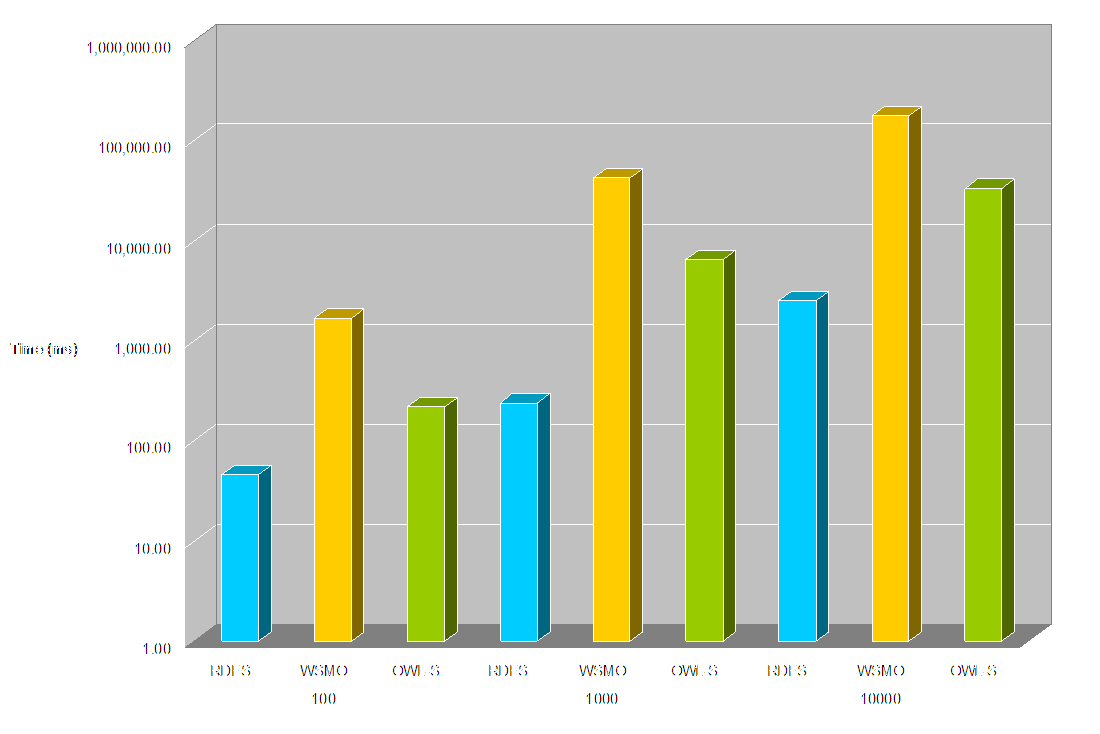
\includegraphics[width=14cm]{images/comparison_chart}
	\caption{Semantic Web Technologies Performance Comparison}
\end{center}
\end{figure}

It can be seen that RDFS performs rather well, even in the 10.000 size set, whereas the other two are pretty far behind. E.g., average response times for WSMO is > 1.5 sec already for the smallest 100 size set. Hence, based on this evaluation the approach to follow for the implementation was RDFS, since WSMO and OWL-S simply could not give the performance required for the real-time discovery.


\clearpage
\section*{Appendix B. Generic building block JSON structure}
\label{appendix_b}
\addcontentsline{toc}{section}{Appendix B. Generic Building Block JSON Structure}

\singlespacing
\begin{verbatim}
{
  "code": "http://url.com/.../code.js",
  "creationDate": "2011-04-20T17:00:00+0100",
  "creator": "username",
  "description": {"en-gb": "This is a description of the building block"},
    "tags":[
      {
        "label":{"en-gb":"Amazon"},
        "means":"http://dbpedia.org/page/Amazon.com"
      },
      {
        "label":{"en-gb":"eBay"},
        "means":"http://dbpedia.org/page/Ebay"
      }
    ],
  "homepage": "http://url.com/.../homepage",
  "icon": "http://url.com/images/.../icon.png",
  "id": "Id of the building block", // i.e. 3545
  "label": {"en-gb": "Label or title of the building block"},
  "rights": "http://creativecommons.org/",
  "screenshot": "http://url.com/.../screenshot.jpg",
  "uri": "http://url.com/screens/525",
  "version": "1.0"
}
\end{verbatim}
\doublespacing


\clearpage
\section*{Appendix C. Screen-flow JSON Structure}
\label{appendix_c}
\addcontentsline{toc}{section}{Appendix C. Screen-flow JSON Structure}

\singlespacing
\begin{verbatim}
{
  <GENERIC BUILDING BLOCK JSON>,
  "contains": [
    "http://url.com/screens/clones/72723",
    "http://url.com/screens/clones/20035",
  ],
}
\end{verbatim}
\doublespacing


\clearpage
\section*{Appendix D. Screen JSON structure}
\label{appendix_d}
\addcontentsline{toc}{section}{Appendix D. Screen JSON Structure}

\singlespacing
\begin{verbatim}
{
  <GENERIC BUILDING BLOCK JSON>,
  "postconditions": [[{
    "id": "Id of the building block", // i.e. 3545
    "label": {"en-gb": "Purchase URL"},
    "pattern": "?url
                http://www.w3.org/1999/02/22-rdf-syntax-ns#type
                http://fast.morfeo-project.org/ontologies/amazon#PurchaseURL",
    "positive": true
  }]],
  "preconditions": [[{
    "id": "cart",
    "label": {"en-gb": "A shopping cart"},
    "pattern": "?cart
                http://www.w3.org/1999/02/22-rdf-syntax-ns#type
                http://fast.morfeo-project.org/ontologies/amazon#ShoppingCart",
    "positive": true
  }]],
  "code": "URL of the code",
  "definition": {
    "buildingblocks: [
      {
        "uri": "http://catalogueURL/forms/clones/670238"
        "uri": "http://catalogueURL/operators/clones/213487"
        "uri": "http://catalogueURL/services/clones/38399"
      },
    ]
    "pipes": [
      {
        "from": {
          "buildingblock": "http://catalogueURL/services/clones/38399",
          "condition": "cA"
        },
        "to": {
          "buildingblock": "http://catalogueURL/operators/clones/213487",
          "action": "filter"
          "condition": "cA",
        }
      },
    "triggers": [
      {
        "from": {
          "buildingblock": "http://catalogueURL/forms/clones/670238",
          "name": "refresh"
        },
        "to": {
          "buildingblock": "http://catalogueURL/services/clones/38399",
          "action": "list"
        }
      }
    ]
  }
}
\end{verbatim}
\doublespacing


\clearpage
\section*{Appendix E. Screen Component JSON structure}
\label{appendix_e}
\addcontentsline{toc}{section}{Appendix E. Screen Component JSON Structure}

\singlespacing
\begin{verbatim}
{
  <GENERIC BUILDING BLOCK JSON>,
  "actions": [{
    "name": "filter",
    "preconditions": [[{
      "id": "item",
      "label": {"en-gb": "Ebay List"},
      "pattern": "?item
                  http://www.w3.org/1999/02/22-rdf-syntax-ns#type
                  http://fast.morfeo-project.org/ontologies/amazon#Item",
      "positive": true
    }]],
    "uses": [{
      "id":"cart",
      "uri":"http://fast.morfeo-project.org/ontologies/amazon#ShoppingCart"
    }]
  }],
  "libraries": [{
    "language":"JavaScript",
    "source":"http://url.com/libcode.js"
  }],
  "postconditions": [[{
    "id": "filterEbay",
    "label": {"en-gb": "Ebay List"},
    "pattern": "?eFilter
                http://www.w3.org/1999/02/22-rdf-syntax-ns#type
                http://developer.ebay.com/.../FindItemsAdvanced.html#Request",
    "positive": true
  }]],
  "triggers": ["itemAmazon"]
}
\end{verbatim}
\doublespacing


\clearpage
\section*{Appendix F. Algorithms for building block recommendation}
\label{appendix_f}
\addcontentsline{toc}{section}{Appendix F. Algorithms for building block recommendation}

The Catalogue serves as a metadata repository for the different kind of resources used by the Gadgets in the FAST platform, or so-called building blocks. The number of building blocks stored in the catalogue is arbitrary, and a simple browsing or keyword-based search through the whole catalogue would be not usable if the number is relatively high.

There are two scenarios where the user may be assisted: screen-flow design, and screen design. At screen-flow design, a user needs to find the proper screens to fulfil her goal. At screen design, the scenario is a bit more complex, where different types of building blocks are involved, making screen creation process more challenging. Therefore, the Catalogue includes several mechanisms in order to help in these situations.


\subsection*{F.1 Pre-/post-conditions matching search}

The building blocks are connected (implicit or explicitaly) to each other via their pre- and post-conditions. These connections are guaranteed by a matching method which determine when a pre-condition is satisfied by a post-condition.

At screen-flow or screen design level, the user needs to find new building blocks which may satisfy elements from the canvas. There is a high probability that building blocks which have compatible pre-/post-conditions might be used to accomplish her goal. The goal for the algorithm is to satisfy a set of pre-conditions, which are still not satisfied, of the elements in the canvas. Therefore, this algorithm searches the Catalogue for building blocks which have post-conditions that satisfy in a certain way some or all of these pre-conditions.

\textcolor{red}{TODO: write about inferencing/reasoning done in the Catalogue}


\subsection*{F.2 Planning}

One of the limitations of the pre-/post-conditions matching algorithm is that the output is limited to satisfy a given set of conditions, but the building blocks suggested may include new pre-conditions to be satisfied, where the user has to add building blocks iteratively until the goal is accomplished (screen-flow or screen is executable).

A set of screens can be seen as a graph (see Figure~\ref{fig:screens_graph}), where the vertices (or nodes) are the screens, and the edges represent whether a screen satisfies or is satisfied by another screen (the arrow points towards the screen which gets satisfied). There is a special node connected to all the screens with no pre-conditions (those are reachable by default). For a given screen, a plan is the path from itself to the special node. These paths or plans are then offered to the user as a set of screens which makes a specific screen reachable.

\begin{figure}[htb]
\label{fig:screens_graph}
\begin{center}
	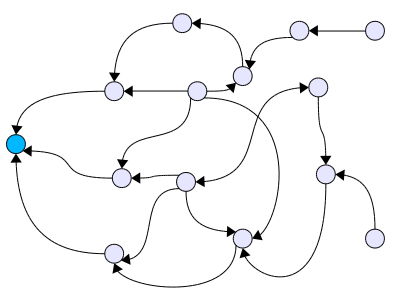
\includegraphics{images/screens_graph}
	\caption{Graph of compatible screens by pre-/post-conditions}
\end{center}
\end{figure}

If the number of vertices and edges is high, the number of different paths can be as well high. This causes problems such as a huge number of different paths between two vertices, or paths which are incredible long, in other words, the number of results or their quality may not be appropiate to be presented to the user, which may expect a few results and with the minimum number of screens as possible. This is a common problem, and there  are many algorithms which solve it, such as Dijkstra or the A* search algorithm which are complete and will always find a solution if one exists.

Our approach has been to implement the A* algorithm, as it calculates a heuristic estimate of the distance to the goal for each node, apart from the path-cost function also included in Dijkstra. In our case, the cost for all edges is the same, and the heuristic function is used to prioritize the screens which are being used already by a given canvas. This way, we try to minimise the number of screens to be used.


\subsection*{F.3 Association Rule Mining}

Association Rule Mining is a well known method for the discovery of relations between variables in large databases. Given a set of transactions, find rules that will predict the occurrence of an item based on the occurrences of other items in the transaction. For example, the rule \verb|{onions, potatoes} = {burger}| found in the sales data of a supermarket would indicate that if a customer buys onions and potatoes together, he or she is likely to also buy burger. 

This method is divided in two steps: frequent itemset mining and rule generation. There are many algorithms for frequent itemset mining as Apriori, Eclat and FP-Growth. This is still a computationally expensive task, and when a mined dataset has a considerable size it is resource intensive \cite{Han:2000:MFP:335191.335372}. However, FP-Growth has demostrated to execute faster than the rest, which lead the open source project called Mahout\footnote{http://mahout.apache.org/} to create its parallel implementation of the algorithm \cite{Li:2008:PPF:1454008.1454027}.

We are not reinventing the wheel doing our own implementation of any algorithm for frequent pattern mining. We opted for integrating the Catalogue with Mahout to make uses of its power, and its scalability advantages.

This algorithm is used both in screen-flow design and screen-design. The approach is similar in both cases, finding building blocks which co-ocurrence is high.

As an example, given the following set of screen-flows:

\begin{table}[h]
\begin{center}
\begin{tabular}{|p{3.5cm}|p{10cm}|}
\hline
\rowcolor{fast@lightgrey}\textcolor{white}{Screen-flow} &
                         \textcolor{white}{Screens} \\ \hline
screenflow-A & screen-1, screen-2 \\ \hline
screenflow-B & screen-1, screen-3, screen-4 \\ \hline
screenflow-C & screen-1, screen-4 \\ \hline
screenflow-D & screen-4, screen-5, screen-7, screen-8 \\ \hline
screenflow-E & screen-3, screen-4, screen-9 \\ \hline
screenflow-F & screen-5, screen-7, screen-2 \\ \hline
screenflow-G & screen-10, screen-11, screen-5, screen-7 \\ \hline
screenflow-H & screen-1, screen-2, screen-3 \\ \hline
\end{tabular}
\end{center}
\end{table}

The algorithm will search for the screens with the highest co-ocurrence for a given input, i.e. a screen-flow during its design phase. For example, for a screen-flow which contains the screen-5, the algorithm will recommend screen-7 as its co-ocurrence is high.

However, the algorithm used for the operations Find \& Check at screen-flow and screen design, is a combination of the pre-/post-conditions matching and frequent itemset mining algorithms. The output items of the frequent itemset mining algorithm are ranked depending on their co-ocurrence, adding the output of the pre-/post-conditions matching search algorithm as if their co-ocurrence was one.


\subsection*{F.4 iServe platform integration}

\textcolor{red}{TODO: write this section}

\end{document}
